\newpage
\section{Lecture 2}
In the previous sections, we considered the case of mass points which continuously interact with each other according to the equations of motion \eqref{1.1a}. It is frequently convenient to consider limiting cases in which the system has only discrete interactions with finite impulses (hard collisions); in such a case the forces are not describable by means of ordinary functions and the Liouville equation must be handled differently. The limiting case of hard collision is useful because it gives a more intuitive idea of the evolution of the system, and it is a good approximation to the strong repulsive forces which actual molecules mutually exert when they are close to each other. 

These considerations lead to the concept of a gas of \textbf{hard spheres}, that is a system of many ``billiard balls'' which do not interact at a distance and collide according to the law of elastic impact. The diameter \(\sigma\) of the spheres is equivalent to the range of force through which actual molecules interact; as a matter of fact a gas of rigid spheres can be pictured as a system of mass points which do not interact when their mutual distance is larger than \(\sigma\), but interact with a formally infinite repulsive central force when the distance is exactly \(\sigma\). 

In the case of a collision between two identical rigid spheres, the equations which relate the velocities after impact \(\vec{\xi}'_1\) and \(\vec{\xi}'_2\) to those before impact, \(\vec{\xi}_1\) and \(\vec{\xi}_2\) are:
\begin{equation}
    \begin{cases}
        \vec{\xi}'_1 = \vec{\xi}_1 - \hat{n} \left[ \hat{n} \cdot \left( \vec{\xi}_1 - \vec{\xi}_2 \right) \right], \\ 
        \vec{\xi}'_2 = \vec{\xi}_2 - \hat{n} \left[ \hat{n} \cdot \left( \vec{\xi}_2 - \vec{\xi}_1 \right) \right],
    \end{cases}
    \label{4.3}
\end{equation}
where \(\hat{n}\) is the unitary vector directed along the line joining the two centers of the spheres.

Next, we will show that the Liouville theorem (conservation of volume in phase space) remains valid for the instantaneous interactions considered here. Instead, in the following we will consider the heuristic arguments proposed by Boltzmann to write an evolution equation for the one-particle probability density \(P^{(1)}(\vec{x}, \vec{\xi}, t)\).

Let us first consider the meaning of \(P^{((1))}(\vec{x}, \vec{\xi}, t)\); it gives the probability density of finding one fixed particle (say the one labeled with \((1)\)) at a certain point \((\vec{x}, \vec{\xi})\) of the \(6\)-dimensional reduced phase space associated with the position and velocity of the particle. We assume that the molecules are hard spheres, whose center has position \(\vec{x}\). The velocities after impact \(\vec{\xi}'_1\) and \(\vec{\xi}'_2\) are related to those before the impact \(\vec{\xi}_1\) and \(\vec{\xi}_2\), by \eqref{4.3}. In the absence of collisions, \(P^{(1)}\) would remain unchanged along the trajectory of the particle.

Accordingly, we must evaluate the effects of collisions on the time evolution of \(P^{(1)}\). Note that the probability of occurrence of a collision is related to the probability of finding another molecule with a center at exactly \(\sigma\) from the particle under observation. 

\begin{wrapfigure}{r}{0.4\textwidth}
    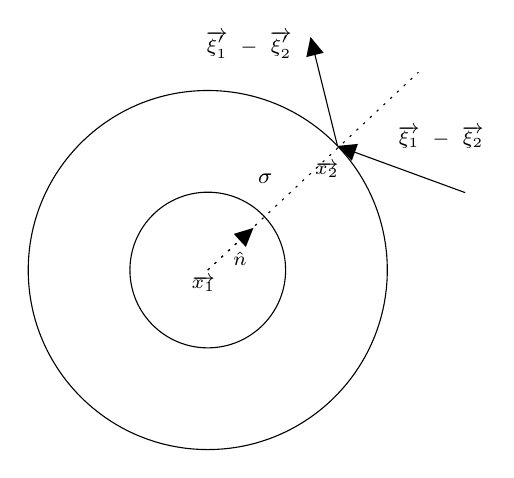
\begin{tikzpicture}[x=0.75pt,y=0.75pt,yscale=-1,xscale=1]
    %uncomment if require: \path (0,240); %set diagram left start at 0, and has height of 240

    %Shape: Circle [id:dp23493641898951367] 
    \draw   (78.5,134) .. controls (78.5,86.23) and (117.23,47.5) .. (165,47.5) .. controls (212.77,47.5) and (251.5,86.23) .. (251.5,134) .. controls (251.5,181.77) and (212.77,220.5) .. (165,220.5) .. controls (117.23,220.5) and (78.5,181.77) .. (78.5,134) -- cycle ;
    %Shape: Circle [id:dp39413567417323714] 
    \draw   (127.5,134) .. controls (127.5,113.29) and (144.29,96.5) .. (165,96.5) .. controls (185.71,96.5) and (202.5,113.29) .. (202.5,134) .. controls (202.5,154.71) and (185.71,171.5) .. (165,171.5) .. controls (144.29,171.5) and (127.5,154.71) .. (127.5,134) -- cycle ;
    %Straight Lines [id:da692567416798913] 
    \draw  [dash pattern={on 0.84pt off 2.51pt}]  (165,134) -- (266.5,38.7) ;
    %Straight Lines [id:da874555083460622] 
    \draw    (289,96.7) -- (230.32,75.23) ;
    \draw [shift={(227.5,74.2)}, rotate = 20.1] [fill={rgb, 255:red, 0; green, 0; blue, 0 }  ][line width=0.08]  [draw opacity=0] (8.93,-4.29) -- (0,0) -- (8.93,4.29) -- cycle    ;
    %Straight Lines [id:da35388877789005657] 
    \draw    (227.5,74.2) -- (215.22,24.61) ;
    \draw [shift={(214.5,21.7)}, rotate = 76.09] [fill={rgb, 255:red, 0; green, 0; blue, 0 }  ][line width=0.08]  [draw opacity=0] (8.93,-4.29) -- (0,0) -- (8.93,4.29) -- cycle    ;
    %Straight Lines [id:da4466205286733381] 
    \draw  [dash pattern={on 0.84pt off 2.51pt}]  (165,134) -- (184.8,115.73) ;
    \draw [shift={(187,113.7)}, rotate = 137.3] [fill={rgb, 255:red, 0; green, 0; blue, 0 }  ][line width=0.08]  [draw opacity=0] (8.93,-4.29) -- (0,0) -- (8.93,4.29) -- cycle    ;

    % Text Node
    \draw (188,86.4) node [anchor=north west][inner sep=0.75pt]  [font=\footnotesize]  {$\sigma $};
    % Text Node
    \draw (156,135.5) node [anchor=north west][inner sep=0.75pt]  [font=\scriptsize]  {$\overrightarrow{x_{1}}$};
    % Text Node
    \draw (215.5,80.5) node [anchor=north west][inner sep=0.75pt]  [font=\scriptsize]  {$\overrightarrow{x_{2}}$};
    % Text Node
    \draw (255.5,63.5) node [anchor=north west][inner sep=0.75pt]  [font=\scriptsize]  {$\overrightarrow{\xi _{1}} \ -\ \overrightarrow{\xi _{2}}$};
    % Text Node
    \draw (163,17.5) node [anchor=north west][inner sep=0.75pt]  [font=\scriptsize]  {$\overrightarrow{\xi '_{1}} \ -\ \overrightarrow{\xi '_{2}}$};
    % Text Node
    \draw (176,123.85) node [anchor=north west][inner sep=0.75pt]  [font=\scriptsize]  {$\hat{n}$};


    \end{tikzpicture}

    \caption{Example of a collision}
\end{wrapfigure}

Thus, in order to write the evolution equation for \(P^{(1)}\) we shall need another equation \(P^{(2)}\) which gives us the probability of finding one particle in \((\vec{x}_1, \vec{\xi}_2)\) and the other in \(\vec{x}_2, \vec{\xi}_2\). Obviously: \(P^{(2)} = P^{(2)}(\vec{x}_1, \vec{x}_2, \vec{\xi}_1, \vec{\xi}_2, t)\).
Hence, \(P^{(1)}\) satisfies an equation of the following form:
\begin{equation}
    \partialderivative{P^{(1)}}{t} + \vec{\xi}_1 \cdot \partialderivative{P^{(1)}}{\vec{x}_1} = G - L.
    \label{1.2.4}
\end{equation}\(L\,d\vec{x}_1 d \vec{\xi}_1 dt\) gives the expected number of particles with position between \(\vec{x}_1\) and \(\vec{x}_1 + d\vec{x}_1\) and velocity between \(\vec{xi}_1 + d\vec{\xi}_1\) that disappear from those range of values because of a collision in the time interval between \(t\) and \(t+dt\), and \(G\,d\vec{x}_1 d \vec{\xi}_1 dt\) gives the number of particles that, instead, enter the same range. 

Counting these numbers is easy, provided we use the trick of imagining particle \(1\) as a sphere at rest and endowed with twice the actual diameter \(\sigma\) and the other particles to be mass points with velocity \((\vec{\xi}_i - \vec{\xi}_1) = \vec{V}_i\) (relative velocity).



In fact, each collision will send particle \(1\) out of the above range and the number of collisions of that particle will be the number of expected collisions of any other particle with that sphere. Since there are exactly \((N-1)\) identical mass points and multiple collisions are disregarded, \(G = (N-1)g\) and \(L = (N-1)l\), where the lowercase letters indicate the contribution of a fixed particle, for example particle \(2\). We shall then compute the effect of collisions of particle \(2\) with particle \(1\). 

Let \(\vec{x}_2\) be a point of the sphere such that the vector joining the center of the sphere with \(\vec{x}_2\) is \(\sigma \hat{n}\), where \(\hat{n}\) is a unit vector. 